\chapter{\label{signal_background}Signal and Background}
% \begin{itemize}
%     \item Write about the how the smaples are generated 
%     \item How you applied the cuts 
%     \item how the DNN are [erforming for the background and signal separation?
%     \item discuss about the vaialbes.    
% \end{itemize}


Monte Carlo simulations are used to model pp collisions at the LHC. Various processes are generated based on their cross sections, kinematics and the dynamics of interaction. MC samples for both signal and background events were produced by the CMS generator team. 
The signal process, pp $\longrightarrow$ $T{^’}$bq, is generated at leading order using the Monte Carlo (MC) event generator MADGRAPH5\_AC@NLO 2.3.3 \cite{Alwall2014, Artoisenet2013}for various masses of of $T{^’}$ quark and for the decay $T{^'}\longrightarrow tH$. The decay of Higgs boson(H$\longrightarrow \gamma \gamma$) is simulated using PYTHIA 8.2 \cite{SJOSTRAND2015159}. The $T{^’}$ quark masses used for final results range from 600 to 1200 GeV. The mass of the Higgs boson is set to 125 GeV and the mass of the top quark is set to 172.5 GeV. The NNPDF3.0 parton distribution function is used \cite{Ball_2015} . The signal samples are generated for left-handed chirality of $T{^’}$ quark. The simulated signal samples with their cross section can be seen in the \autoref{tab:my_labeL_Signal} \\
As for background MC samples, various generators are exploited: MADGRAPH5\_AMC@NLO 2.2.2 (MG5\_AMC), PYTHIA 8.2\cite{SJOSTRAND2015159}, SHERPA 2.2 \cite{10.21468/SciPostPhys.7.3.034}. For the 2016 MC production, the PYTHIA tune CUETP8M1 \cite{Khachatryan2016} is used, while for the 2017 and 2018 MC productions, the PYTHIA tune CP5 \cite{Sirunyan2020} is adopted. \\
Two types of SM background are considered according to their shapes in the di-photon invariant mass spectrum: resonant background (SMH) and non-resonant background (NRB). The former refers to the SM Higgs production processes while the latter refers to other SM processes that have non-negligible contributions to the analysis. The simulated background samples with their cross section can be seen in the \autoref{tab:my_label_BAckground}\\
The major SM Higgs production modes are produced with MG5 a MC@NLO interfaced with PYTHIA 8.2, including gluon fusion \cite{Bagnaschi_2012}, vector boson fusion, production in association with with top quarks \cite{PhysRevD.91.094003}, and with a vector boson. The total cross-sections and branching ratios recommended by the LHC cross-section working group  are used.


For the non-resonant background, di-photon samples, in which two prompt photons not forming a peak, are simulated by SHERPA 2.2. QCD multi-jets events (contributing two fake photons) and gamma + jets processes (offering one prompt photon and one fake photons) are simulated by PYTHIA 8.2, with a ”Double EM-enriched” filter applied during production. 


After generation, events are propagated through the simulation of the CMS detector using the
Geant4\cite{AGOSTINELLI2003250} package. The effects of multiple proton-proton interactions are also modeled in the
package by adding simulated minimum-bias interactions to the simulated samples. The number of pileup interactions agrees with the one observed in data after reweighting the simulated pileup distribution, with the recommended 69.2 mb minimum bias cross-section.


\begin{table}[H]
    \centering
    \resizebox{\textwidth}{!}{
    \begin{tabular}{|c|c|c|} \hline
     Sample Name    & $T^'$ Mass  & Cross-Section(fb) \\
                    & (${GeV}/{c^2}$) & 13TeV\\ \hline
 TprimeBToTH\_Hgg\_M-600\_LH\_TuneCP5\_PSweights\_13TeV-madgraph\_pythia8.root    &  600 & 1.161 \\
 TprimeBToTH\_Hgg\_M-625\_LH\_TuneCP5\_PSweights\_13TeV-madgraph\_pythia8.root    & 625 & 0.939 \\
 TprimeBToTH\_Hgg\_M-650\_LH\_TuneCP5\_PSweights\_13TeV-madgraph\_pythia8.root    & 650 & 0.717 \\
 TprimeBToTH\_Hgg\_M-675\_LH\_TuneCP5\_PSweights\_13TeV-madgraph\_pythia8.root  & 675 & 0.586  \\
 TprimeBToTH\_Hgg\_M-700\_LH\_TuneCP5\_PSweights\_13TeV-madgraph\_pythia8.root    & 700  & 0.455 \\\hline \hline
 TprimeBToTH\_Hgg\_M-800\_LH\_TuneCP5\_PSweights\_13TeV-madgraph\_pythia8.root    & 800 & 0.196\\
  TprimeBToTH\_Hgg\_M-900\_LH\_TuneCP5\_PSweights\_13TeV-madgraph\_pythia8.root   & 900  & 0.0903 \\
  TprimeBToTH\_Hgg\_M-1000\_LH\_TuneCP5\_PSweights\_13TeV-madgraph\_pythia8.root   & 1000  &  0.0440\\ \hline \hline
  TprimeBToTH\_Hgg\_M-1100\_LH\_TuneCP5\_PSweights\_13TeV-madgraph\_pythia8.root  & 1100  &   0.0224 \\
  TprimeBToTH\_Hgg\_M-1200\_LH\_TuneCP5\_PSweights\_13TeV-madgraph\_pythia8.root   &  1200  & 0.0118	\\ \hline
    \end{tabular}}
    \caption{List of Monte Carlo signal samples used in the analysis with their cross-section\cite{CrossSection_1}. }
    \label{tab:my_labeL_Signal}
\end{table}



\begin{table}[H]
    \centering
    \resizebox{\textwidth}{!}{
    \begin{tabular}{|c|c|c|} \hline
    Standard Model Higgs background    & Cross-Section \\
                   & $\times$ BR(H$\longrightarrow \gamma \gamma$)(fb)\\ \hline
  ttHJetToGG\_M125\_13TeV\_amcatnloFXFX\_madspin\_pythia8.root   &  1.15 \\
   THQ\_ctcvcp\_HToGG\_M125\_13TeV-madgraph-pythia8.root & 0.17 \\   
 GluGluHToGG\_M125\_TuneCP5\_13TeV-amcatnloFXFX-pythia8.root & 110.28 \\  
 VBFHToGG\_M125\_13TeV\_amcatnlo\_pythia8.root  &  8.59 \\
VHToGG\_M125\_13TeV\_amcatnloFXFX\_madspin\_pythia8.root & 5.12\\\hline \hline
   Non-resonant background      &    Cross-Section (pb)  \\ \hline
   output\_TTJets\_pythia8.root   &     722.8 \\ 
   output\_TTGG\_0Jets\_pythia8.root  &  0.01687\\
   output\_TGJets\_pythia8.root  &  2.967  \\
   output\_GJet\_Pt-40toInf\_DoubleEMEnriched\_MGG-80toInf\_pythia8.root & 878.1\\
   output\_DiPhotonJetsBox\_MGG-80toInf\_13TeV-Sherpa.root    &   84.4  \\\hline
    \end{tabular}}
    \caption{List of background samples. \cite{crossSection_2, crossSection_3}}
    \label{tab:my_label_BAckground}
\end{table}

\section{ Physics Objects}
\subsection{Primary Vertex Selection}
Events to analyze should satisfy the following conditions:
\begin{itemize}
    \item At least one good primary vertex with n.d.o.f. $\geq$4.
    \item The track impact parameter with respect to the beam spot on the z axis, |z| , should be within 24 cm
    \item The track impact parameter with respect to the beam spot on the x-y plane, |$\rho$|, should be smaller than 2 cm
\end{itemize}

\subsection{Photons}
Photons are reconstructed with the energy deposits of the electromagnetic calorimeter (ECAL). Not associated with the tracker's charged particle track due to incomplete simulation, detection effect and energy loss correction by converted photons in  tracker by considering the following physical quantities:
\begin{itemize}
    \item Shower shape and isolation variables
    \item Energy scales and smearing
\end{itemize}


Photon identification MVA is an important algorithm used to isolate ("prompt") photons and false photons in a jet from quark / gluon fragmentation and hadronization. Training is  based on DNN(Deep Neural Network) and BDT(Boosted Decision Trees) using simulated samples. 
 Analysis of $\gamma$+ jets events using prompt photons  as signals while using fake photons from jets as a background. The training takes the corrected shower shape and isolation variables as the input features. 
 
 
 In the analysis, any two photons in an events forms a di-photon candidates. For each di-photon candidate, $p_T$ cuts  are imposed for the leading (sub-leading) photon to maintain a smooth shape of the $m_{\gamma\gamma}$ distribution. Since $\frac{p_T}{m_{\gamma\gamma}}$ has a dependency on the opening angle between two photons, imposing the $\frac{p_T}{m_{\gamma\gamma}}$ can prevent a bad resolution of diphoton invariant mass as well \autoref{eq:equation_6}. This selection is standard in the H$\longrightarrow \gamma\gamma$ analysis.
 
 \begin{equation}\label{eq:equation_6}
     m_{\gamma_1\gamma_2} = \sqrt{E_{\gamma_1}E_{\gamma_2}(1- \cos{\theta_{\gamma_1\gamma_2}})}
 \end{equation}
 
 For each photon, photon ID MVA score is required to be larger than − 0.7, which eliminates
reducible background events without loosing much VLQ signal events in the H$\longrightarrow \gamma\gamma$ channel.
If there are more than one di-photon candidate surviving all the event selections in an event, the candidate with the largest scalar sum of two photons $p_T$ is chosen as the Higgs candidate of the event.

Invariant mass of the leading two photons is further used to define the signal window and the sideband regions:
\begin{itemize}
    \item Signal window: $m_{\gamma\gamma} \in$ [115, 135]GeV
    \item Sideband region: $m_{\gamma\gamma} \in$ [110, 115] $\cup$ [135, 180]GeV.
\end{itemize}
The signal window is blinded throughout the development of the analysis.

\subsection{Jets}

We follow the standard recommendations from JetMET physics object group for treatments of jets. Reconstruction of jets is based on anti-kT clustering algorithm \cite{Cacciari_2008} with a distance parameter being 0.4 (AK4). The jets originate from particle flow candidates with charged hadron coming from non-primary vertices subtracted (PFchs). The jet energy corrections and energy smearing are applied according to the recipes provided by the JERC group\cite{CrossSection_5}.

\subsection{b-tagged jets}
Jets originating from the hadronization of b-quarks are tagged using the DeepCSV algorithm. The loose working point of the DeepCSV algorithm is used to identify b jets. Addition-
ally, the b jets are required to be in the barrel region ( | $\eta$ | < 2.5). 


\subsection{Missing ET}
The missing transverse momentum vector $\Bar{P_T}^ {miss}$ is computed as the negative vector sum of the transverse momenta of all the PF candidates in an event. The magnitude of $\Bar{P_T}^ {miss}$ is denoted as MET. In the analysis, MET considers the standard type 1 correction (JEC propagation) while the variation of MET uncertainty considers effects from JEC and unclustered energy.

The different variable used in this analysis are listed in \autoref{tab:my_label_Variable}

  \begin{table}[h!]
    \centering
    \resizebox{6cm}{!}{
    \begin{tabular}{|c|c|}\hline
     Sl. No.    & Variables \\\hline
       1  & dipho\_leadPt \\
        2  & dipho\_mass\\
         3  & dipho\_leadEta \\
          4  & dipho\_leadIDMVA \\
           5  & dipho\_subleadIDMVA \\
            6  & dipho\_lead\_haspixelseed \\
             7  & dipho\_sublead\_haspixelseed \\
              8  & n\_jets \\
               9  & n\_bjets \\
                10  & n\_centraljets \\
                 11  & lepton\_charge \\
                  12  & lepton\_leadPt \\
                   13  & lepton\_leadEta \\
                    14  & fwdjet1\_pt \\
                     15  & fwdjet1\_eta \\
                      16  & fwdjet1\_discr \\
                       17  & top\_mt\\
                        18  & dr\_tHchainfwdjet \\
                         19  & dr\_leptonbjet \\
                          20  & dr\_leptonfwdjet\\
                          21  & dr\_bjetfwdjet \\
                            22  & dr\_leadphofwdjet\\
                             23  & dr\_subleadphofwdjet \\
                              24  & bjet1\_pt\\
                              25 & bjet2\_pt \\
                              26  & bjet3\_pt \\
                               27 & bjet1\_eta \\
                              28  & bjet2\_eta \\
                                29  & bjet3\_eta \\
                                  30  & bjet1\_discr\\
                                    31  & bjet2\_discr \\ 
                                    32 & bjet3\_discr \\
                                   33  &   jet1\_pt \\
                                    34  &  jet2\_pt  \\
                                   35    &  jet3\_pt  \\
                                  36      &  jet1\_eta  \\
                                 37        & jet2\_eta   \\
                                 38         &  jet3\_eta  \\
                                    39       &  jet1\_discr  \\
                                      40      &  jet2\_discr  \\
                                       41      &   jet3\_discr \\
                                       42       &  dipho\_subleadEta  \\
                                    
                                    
                                    
                                    \hline
           
    \end{tabular}}
    \caption{Variables of signal and Background used as input variable of the DNN model and further used as testing}
    \label{tab:my_label_Variable}
\end{table}





Even when intriguing particles are created, finding them is a difficult task. They are too tiny to be seen directly and disintegrate into other particles nearly instantly. Although new particles cannot be seen directly, the lighter stable particles to which they decay, known as decay products, can. For this reason, multiple layers of detectors surround the moment of impact. Each decay product interacts with these detectors in a way that permits the direction and momentum of the decay product to be detected. \\
Electrically charged leptons (electrons or muons, designated) and particle jets are visible decay products (collimated streams of particles originating from quarks or gluons, denoted j).


The synthesis of top quarks in pairs ($\Bar{t}tH$)  or singly (tH) with the Higgs boson allows direct experimental access to the top-Higgs interaction with an output signature comparable to that of  $\Bar{t}tH (tH)$ decay. The ttH (tH) production mode has a highly distinctive experimental signature, which includes leptons and/or jets from the decay of the two (single) top quarks, as seen in \autoref{fig:my_label_tth}, while proceeding at a rate roughly 100(1000) times slower than gluon fusion.\\



The ttH production cross section is predicted to grow by a factor of four as the LHC energy is increased from 8 to 13 TeV for Run 2. However, such a mechanism is still uncommon, and searches for ttH creation have been fueled by the increased sensitivity achieved in Higgs decay modes with higher branching fractions. \\
\begin{figure}[H]
    \centering
    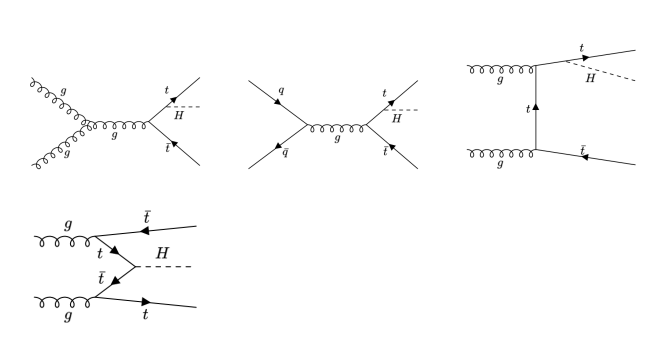
\includegraphics[scale=0.7]{figure_1/tth_1.png}
    \caption{Feynman diagrams depicting $t\Bar{t}H$ production modes}
    \label{fig:my_label_tth}
\end{figure}
The T$^'$ quark could couple to bW, tZ, or tH, resulting in the corresponding T$^'$ quark decays as shown with Feynman diagram in the \autoref{fig:my_label_T'}. All the other few backgrounds with similar decay signature used as the backgrounds are shown in \autoref{fig:my_label_ttgg}, \autoref{fig:my_label_thq}, and \autoref{fig:my_label_ttgg_12}.\\




\begin{figure}[H]
    \centering
    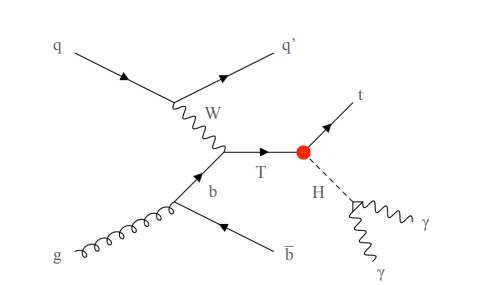
\includegraphics[scale=0.5]{figure_1/T'.png}
    \caption{Leading-order Feynman diagram for single T’ production}
    \label{fig:my_label_T'}
\end{figure}


\begin{figure}[H]
    \centering
    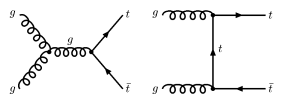
\includegraphics[scale=0.5]{figure_1/ttgg.png}
    \caption{ttgg Feynman diagram}
    \label{fig:my_label_ttgg}
\end{figure}

\begin{figure}[H]
    \centering
    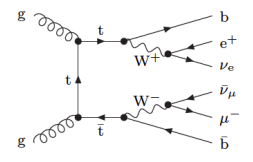
\includegraphics[scale=0.5]{figure_1/ttgg__.png}
    \caption{Feynman diagram for ttgg}
    \label{fig:my_label_ttgg_12}
\end{figure}


\begin{figure}[H]
    \centering
    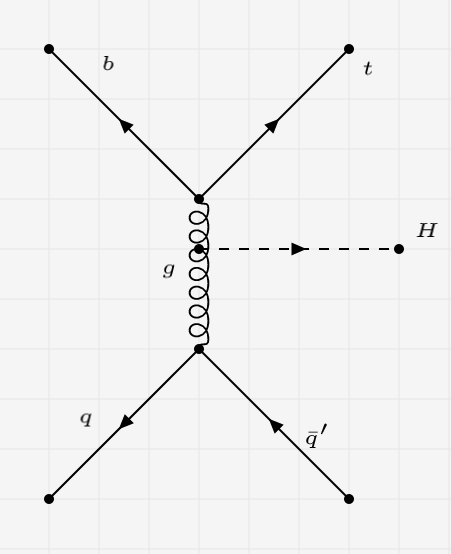
\includegraphics[scale =0.5]{figure_1/thq.png}
    \caption{Feynman diagram of thq}
    \label{fig:my_label_thq}
\end{figure}




Few of the plots of variables of these simulated samples are shown in \autoref{fig:Signal_bkg_plotting} with the high level input features on the right side of \autoref{fig:Signal_bkg_plotting} and low level input features on the left of \autoref{fig:Signal_bkg_plotting}.
\begin{figure}[H]
\begin{subfigure}{.5\textwidth}
  \centering
  % include first image
  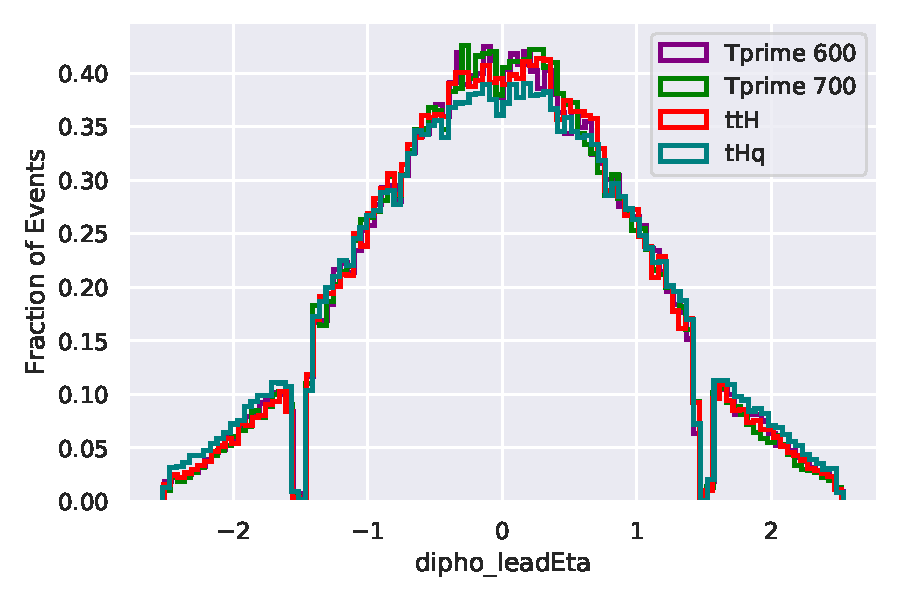
\includegraphics[width=.8\linewidth]{Figure_2/dipho_leadEta.pdf}  
  \caption{}
  \label{fig:sub-first}
\end{subfigure}
\begin{subfigure}{.5\textwidth}
  \centering
  % include second image
  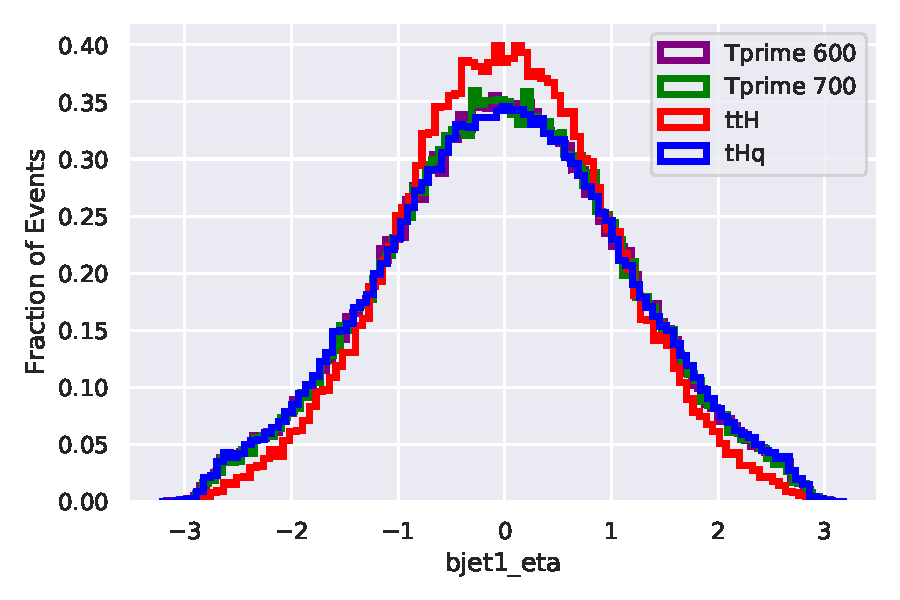
\includegraphics[width=.8\linewidth]{Figure_2/bjet1_eta.pdf}  
  \caption{}
  \label{fig:sub-second}
\end{subfigure}



\begin{subfigure}{.5\textwidth}
  \centering
  % include third image
  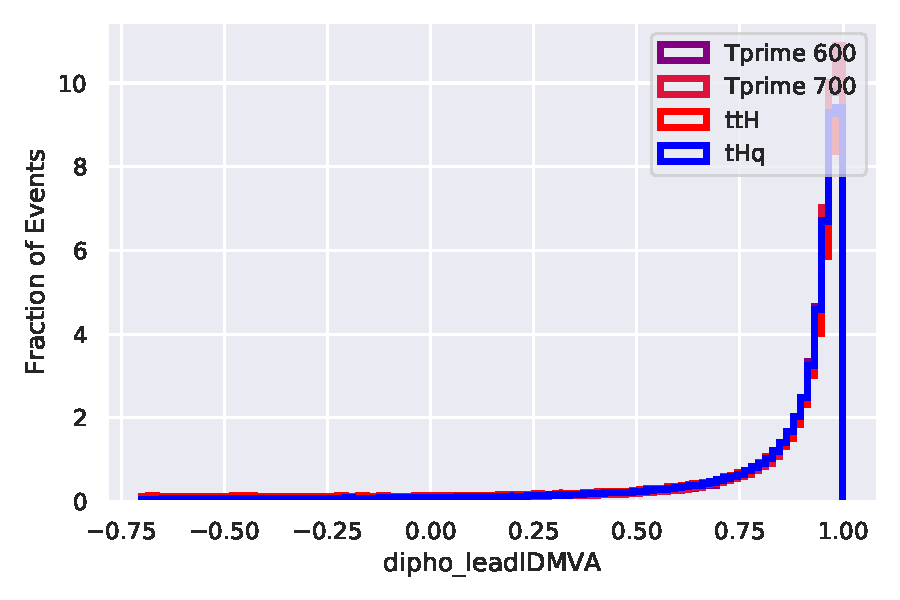
\includegraphics[width=.8\linewidth]{Figure_2/dipho_leadIDMVA.pdf}  
  \caption{}
  \label{fig:sub-third}
\end{subfigure}
\begin{subfigure}{.5\textwidth}
  \centering
  % include fourth image
  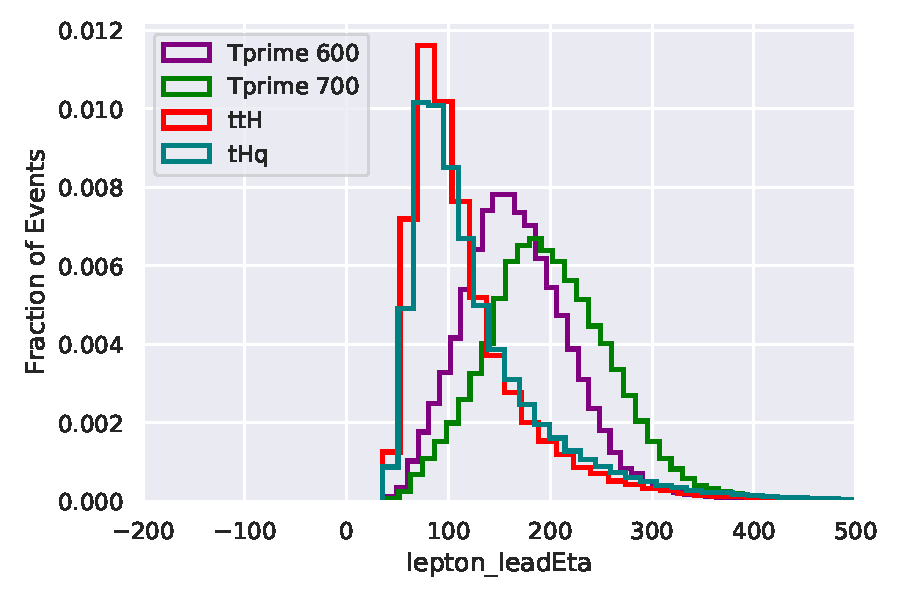
\includegraphics[width=.8\linewidth]{Figure_2/dipho_leadPt.pdf}  
%   \caption{}
  \label{fig:sub-fourth}
\end{subfigure}


\begin{subfigure}{.5\textwidth}
  \centering
  % include third image
  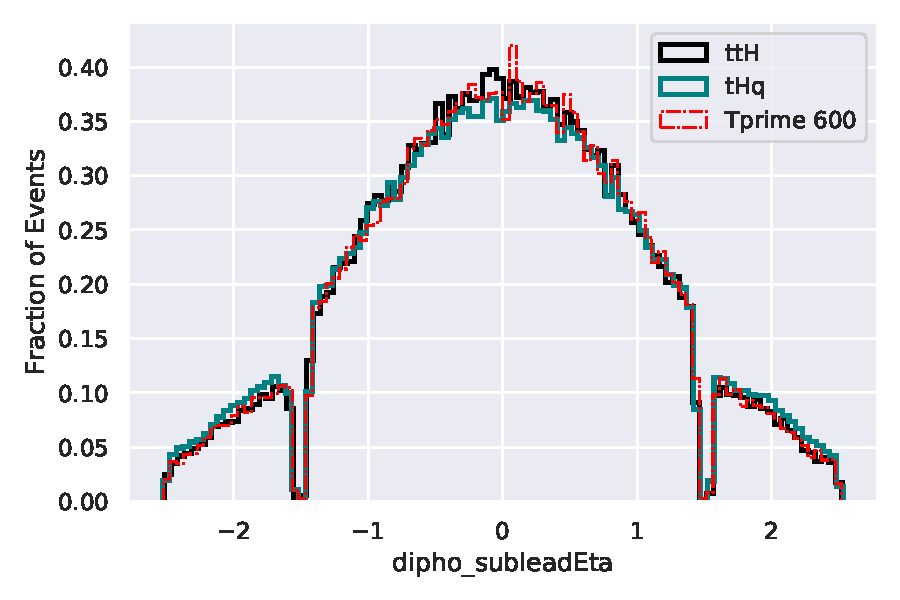
\includegraphics[width=.8\linewidth]{Figure_2/dipho_subleadEta.pdf}  
%   \caption{}
  \label{fig:sub-fifth}
\end{subfigure}
\begin{subfigure}{.5\textwidth}
  \centering
  % include fourth image
  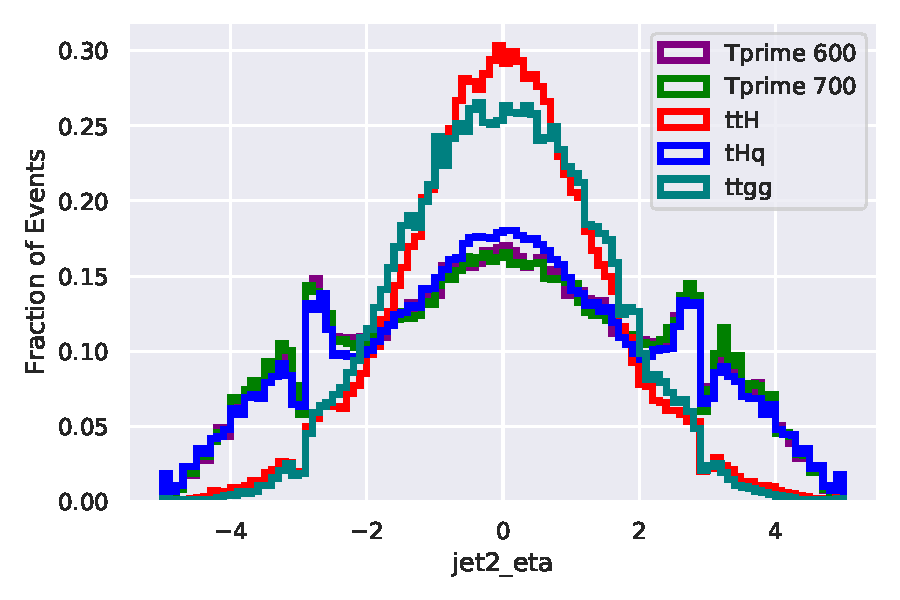
\includegraphics[width=.8\linewidth]{Figure_2/jet2_eta.pdf}  
%   \caption{}
  \label{fig:sub-fourth}
\end{subfigure}

\begin{subfigure}{.5\textwidth}
  \centering
  % include third image
  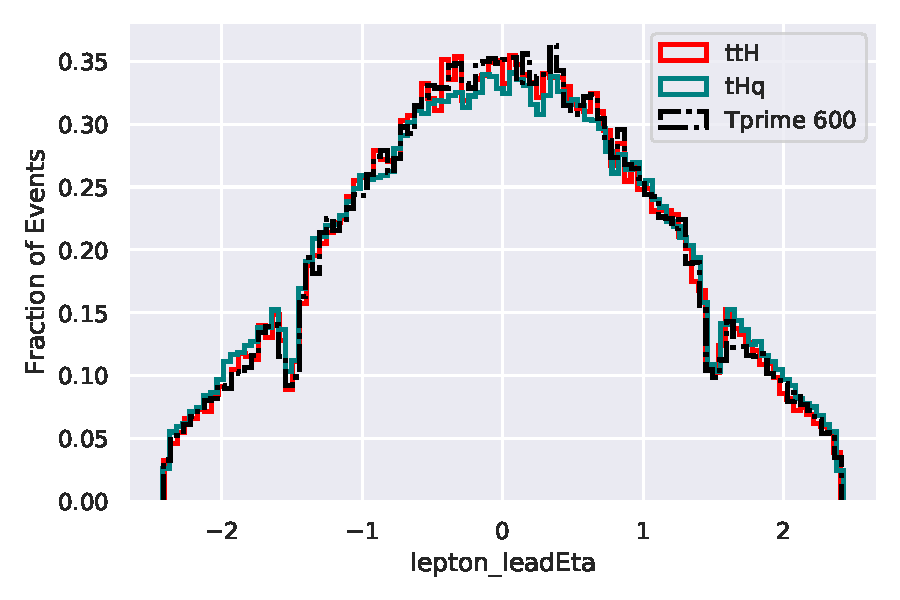
\includegraphics[width=.8\linewidth]{Figure_2/lepton_leadEta.pdf}  
%   \caption{}
  \label{fig:sub-third}
\end{subfigure}
\begin{subfigure}{.5\textwidth}
  \centering
  % include fourth image
  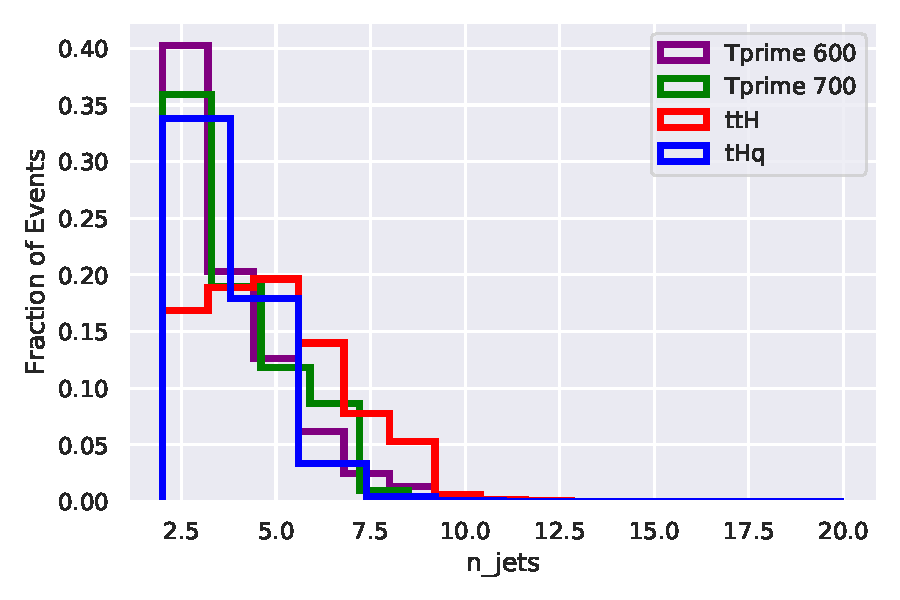
\includegraphics[width=.8\linewidth]{Figure_2/n_jets.pdf}  
%   \caption{}
  \label{fig:sub-fourth}
\end{subfigure}
\caption{Simulated sample plot for different variables, for each figure plotted above the signal is Tprime and the standard model higgs as the background. From top to bottom, plots for different variable are as, (a) Plot for $dipho\_leadEta$, (b) Plot for $bjet1\_eta$, (c)Plot for $dipho\_leadIDMVA$, (d) Plot for $dipho\_leadPt$, (e) Plot for $dipho\_subleadEta$, (f) Plot for $jet2\_eta$, (g) Plot for $lepton\_leadEta$, and (h) Plot for n\_jets  }
\label{fig:Signal_bkg_plotting}
\end{figure}
 
In the given \autoref{fig:Signal_bkg_plotting}, even from the best separation among the input variable of the Tprime(signal) and SMH(background) model of the monte carlo smaples, we cannot see how our signal (Tprime) get clearly separated from the standard model higgs(SMH) backgrounds. 
For the better separation between these two, we need the application of machine learning techniques(DNN), which discussed in details with outputs in \autoref{AN}, \autoref{R_D}.
For the testing for the presence of any signals in the \textit{RUN II} datafile,  the DNN training model have been tested on \textit{"allData\_RunII.root"}, which collected by CMS during 2016, 2017, 2018 run of the LHC, with an integrated
luminosity of 137.65$fb^{-1}$ , is used for this analysis..




% \noindent\fbox{%
%     \parbox{\textwidth}{%
%         1. In the signal hypothesis we expect that: 
%         2. Write what expect in the background hypothesis.
%         3. 
%     }%
% }








\setcounter{equation}{0}
\setcounter{table}{0}
\setcounter{figure}{0}
%\baselineskip 24pt


% %%%%%%%%%%%%%%%%%%%%%%QUESTIONS MAY GET FRAMED FROM HERE%%%%%%%%%%%%%%%%%%%%%%%%%%%%%%%%%%%%%%%%%%%%%%
% \begin{itemize}
%     \item Why we measure luminosity in $fb^{-1}$
% \end{itemize}